\documentclass[11pt,letterpaper]{article}
\usepackage[lmargin=1in,rmargin=1in,tmargin=1in,bmargin=1in]{geometry}
\usepackage{../style/homework}
\usepackage{../style/commands}
\setbool{quotetype}{true} % True: Side; False: Under
\setbool{hideans}{false} % Student: True; Instructor: False

% -------------------
% Content
% -------------------
\begin{document}

\homework{15: Due 11/16}{He is a self-made man and worships his creator.}{Henry Clapp}

% Problem 1
\problem{10} As accurately as possible, plot the function $f(x)= \frac{1}{4} \left( 2^{x - 2} \right)$.
	\[
	\fbox{
	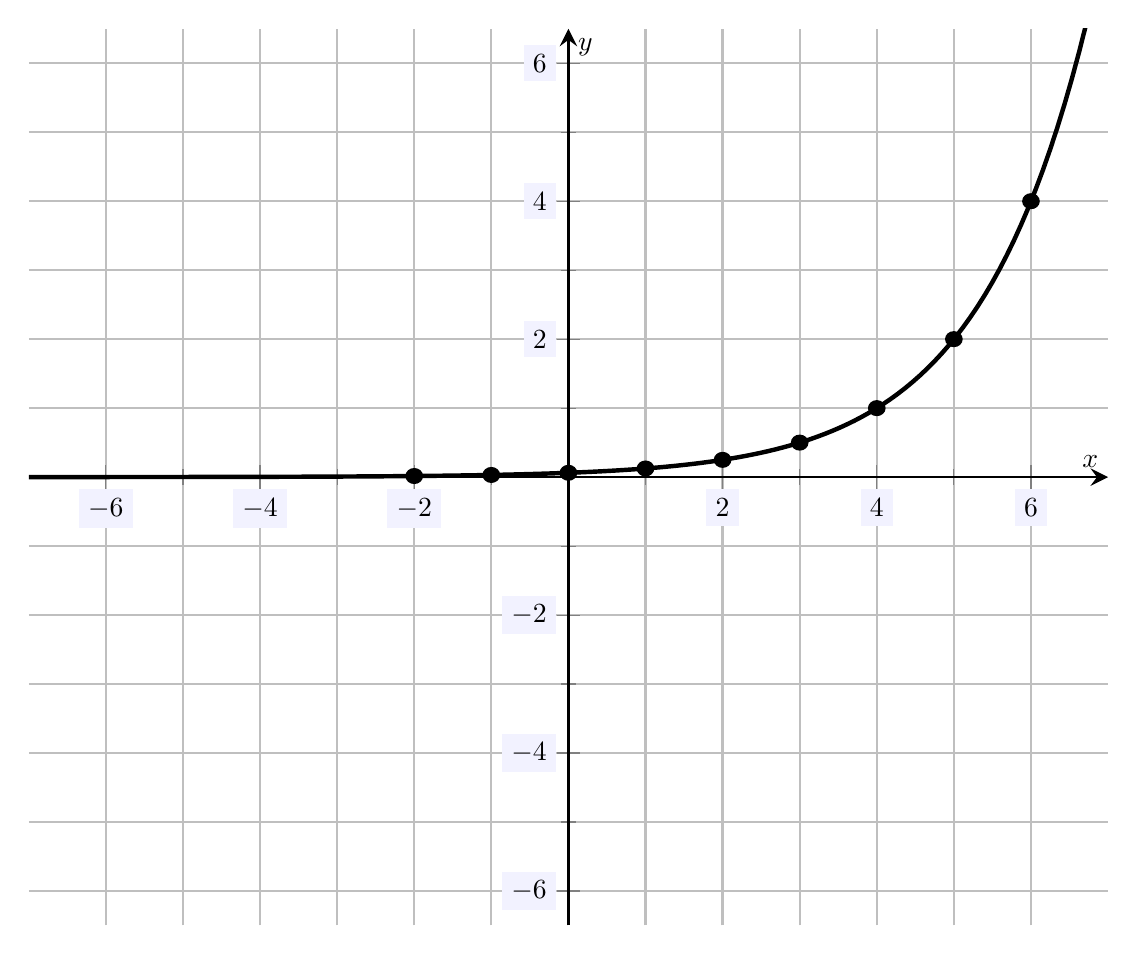
\begin{tikzpicture}[scale=2,every node/.style={scale=0.5}]
	\begin{axis}[
	grid=both,
	axis lines=middle,
	ticklabel style={fill=blue!5!white},
	xmin= -7, xmax=7,
	ymin= -6.5, ymax=6.5,
	xtick={-6,-4,-2,0,2,4,6},
	ytick={-6,-4,-2,0,2,4,6},
	minor tick = {-5,-3,...,5},
	xlabel=\(x\),ylabel=\(y\),
	]
	\addplot[thick, domain= -7:7,samples=150] {1/4*2^(x-2)};
	\draw[fill=black] (-2,1/64) circle (0.1);
	\draw[fill=black] (-1,1/32) circle (0.1);
	\draw[fill=black] (0,1/16) circle (0.1);
	\draw[fill=black] (1,1/8) circle (0.1);
	\draw[fill=black] (2,1/4) circle (0.1);
	\draw[fill=black] (3,1/2) circle (0.1);
	\draw[fill=black] (4,1) circle (0.1);
	\draw[fill=black] (5,2) circle (0.1);
	\draw[fill=black] (6,4) circle (0.1);
	\end{axis}
	\end{tikzpicture}
	}
	\] \pspace

	\begin{table}[!ht]
	\centering
	\begin{tabular}{r||rrrrrrrrr}
	$x$ & $-2$ & $-1$ & $0$ & $1$ & $2$ & $3$ & $4$ & $5$ & $6$ \\ \hline
	$f(x)$ & $\frac{1}{64}$ & $\frac{1}{32}$ & $\frac{1}{16}$ & $\frac{1}{8}$ & $\frac{1}{4}$ & $\frac{1}{2}$ & $1$ & $2$ & $4$
	\end{tabular}
	\end{table}





\newpage





% Problem 2
\problem{10} Sketch a graph of the function $y= 4 (2^{1 - x})$. 
	\[
	\fbox{
	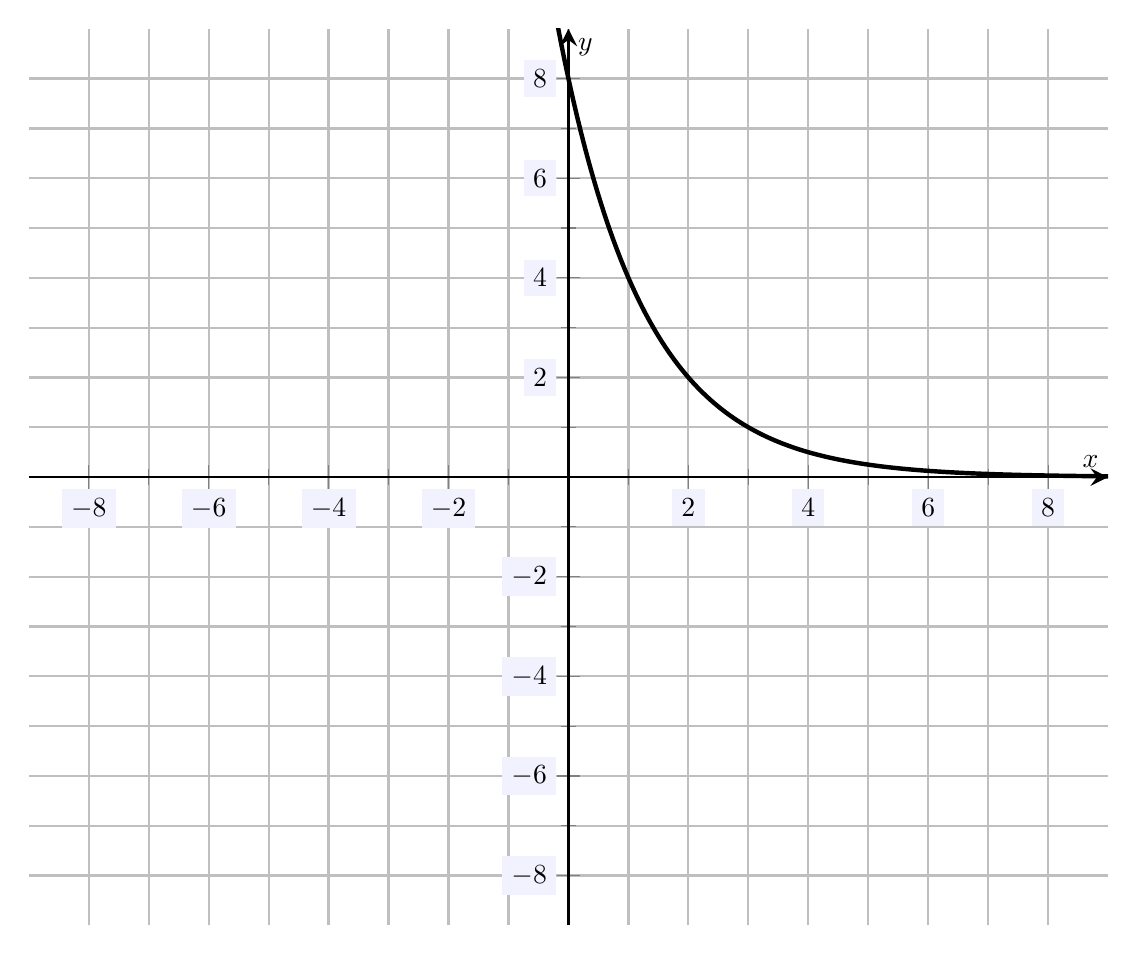
\begin{tikzpicture}[scale=2,every node/.style={scale=0.5}]
	\begin{axis}[
	grid=both,
	axis lines=middle,
	ticklabel style={fill=blue!5!white},
	xmin= -9, xmax=9,
	ymin= -9, ymax=9,
	xtick={-8,-6,-4,-2,0,2,4,6,8},
	ytick={-8,-6,-4,-2,0,2,4,6,8},
	minor tick = {-8,-7,...,8},
	xlabel=\(x\),ylabel=\(y\),
	]
	\addplot[thick, domain= -1:9,samples=150] {4*2^(1-x)};
	\end{axis}
	\end{tikzpicture}
	}
	\] \pspace

Writing $y$ in the form $Ab^x$, we have\dots
	\[
	y= 4(2^{1 - x})= 4(2 \cdot 2^{-x})= 8 (2^{-x})= 8(2^{-1})^x= 8 \left( \dfrac{1}{2} \right)^x
	\] 
Because $b= \frac{1}{2}$, where $0 < b < 1$, and $A= 8 > 0$, the function is decreasing. We have $y$-intercept with $y$-coordinate\dots
	\[
	y(0)= 4(2^{1 - 0})= 4(2)= 8,
	\]
i.e. the $y$-intercept is $(0, 8)$. 





\newpage





% Problem 3
\problem{10} Consider the function $y= -9 (2^{-2x})$.
\begin{enumerate}[(a)]
\item Is the function increasing or decreasing? Explain.
\item Find the $y$-intercept of this function.
\item What are the $x$-intercepts and zeros for this function?
\item Find $y(-1)$. 
\end{enumerate} \pspace

\sol
\begin{enumerate}[(a)]
\item We write $y$ in the form $Ab^x$:
	\[
	y= -9(2^{-2x})= -9(2^{-2})^x= -9 \left( \dfrac{1}{2^2} \right)^x= -9 \left( \dfrac{1}{4} \right)^x
	\]
Because $b= \frac{1}{4}$, where $0 < b < 1$, and $A= -9 < 0$, the function is increasing. \pspace

\item The $y$-intercept occurs when $x= 0$, where then $y$ is\dots
	\[
	y= -9(2^{-2(0)})= -9( 2^0)= -9 \cdot 1= -9
	\]
Therefore, the $y$-intercept is $(0, -9)$. \pspace

\item The function $y= -9(2^{-2x})$ is always negative because $A= -9 < 0$. Therefore, there are no $x$-intercepts (and hence zeros) for the function $y= -9(2^{-2x})$. \pspace

\item 
	\[
	y(-1)= -9(2^{-2(-1)})= -9(2^2)= -9(4)= -36
	\]
\end{enumerate}





\newpage





% Problem 4
\problem{10} Consider the function $y= 3^{1-x} - 9$.
\begin{enumerate}[(a)]
\item Is the function increasing or decreasing? Explain.
\item Find the $y$-intercept of this function.
\item What are the $x$-intercepts and zeros for this function?
\item Find $y(2)$. 
\end{enumerate} \pspace

\sol
\begin{enumerate}[(a)]
\item We write $y$ in the form $Ab^x + C$:
	\[
	y= 3^{1-x} - 9= 3 \cdot 3^{-x} - 9= 3 (3^{-1})^x - 9= 3 \left( \dfrac{1}{3} \right)^x - 9
	\]
Because $b= \frac{1}{3}$, where $0 < b < 1$, and $A= 3 > 0$, the function is decreasing. \pspace

\item The $y$-intercept occurs when $x= 0$, where then $y$ is\dots
	\[
	y(0)= 3^{1 - 0} - 9= 3^1 - 9= 3 - 9= -6
	\]
Therefore, the $y$-intercept is $(0, -6)$. \pspace

\item 
	\[
	\begin{aligned}
	3^{1-x} - 9&= 0 \\[0.3cm]
	3^{1 - x}&= 9 \\[0.3cm]
	3^{1 - x}&= 3^2
	\end{aligned}
	\]
Because the bases on each side are the same, we must have $1 - x= 2$. But then $x= -1$. Therefore, the only zero is $x= -1$. This corresponds to an $x$-intercept of $(-1, 0)$. \pspace

\item 
	\[
	y(2)= 3^{1 - 2} - 9= 3^{-1} - 9= \dfrac{1}{3} - 9= \frac{1}{3} - \dfrac{27}{3}= -\dfrac{26}{3}
	\]
\end{enumerate}


%\printpoints
\end{document}